\documentclass{beamer}

\usepackage[utf8]{inputenc}
\usepackage{hyperref}

\usetheme{Berkeley}
\beamertemplatenavigationsymbolsempty
\setbeamertemplate{headline}{}
 
\title{Geo-Clustering in FoodChain-Lab}
\date{}
 
\begin{document}
\maketitle

\section{ }

\subsection{Task}
\begin{frame}
	\begin{itemize}
		\item Perform a clustering base the following workflow: \url{https://github.com/SiLeBAT/BfROpenLabResources/raw/master/GitHubPages/workflows/Example_Workflow.zip}
		\item Cluster all French stations by using the \textbf{GIS Cluster} node.
		\item Use a \textbf{Max Neighborhood Distance} of 100km.
		\item That means two stations are put into the same cluster if their distance if less than 100km.
	\end{itemize}
\end{frame}
 
\subsection{1}
\begin{frame}
	\begin{center}
  		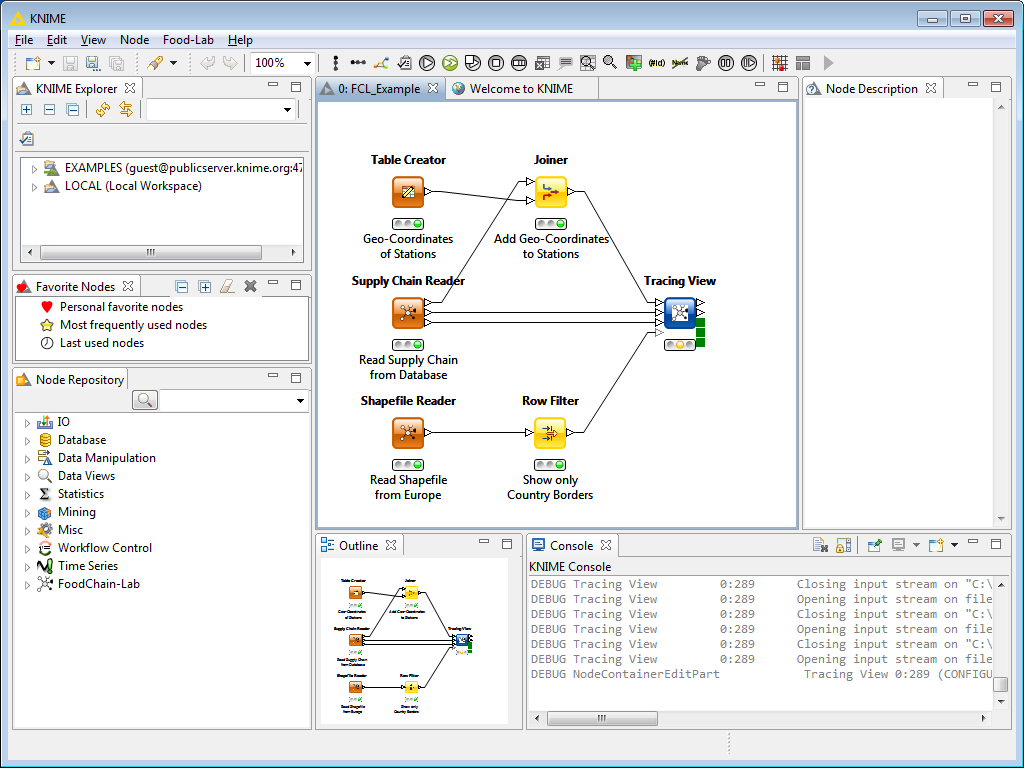
\includegraphics[height=0.6\textheight]{1.png}
	\end{center}
	\begin{itemize}
		\item Import the Example Workflow from \url{https://github.com/SiLeBAT/BfROpenLabResources/raw/master/GitHubPages/workflows/Example_Workflow.zip}.
	\end{itemize}
\end{frame}

\subsection{2}
\begin{frame}
	\begin{center}
  		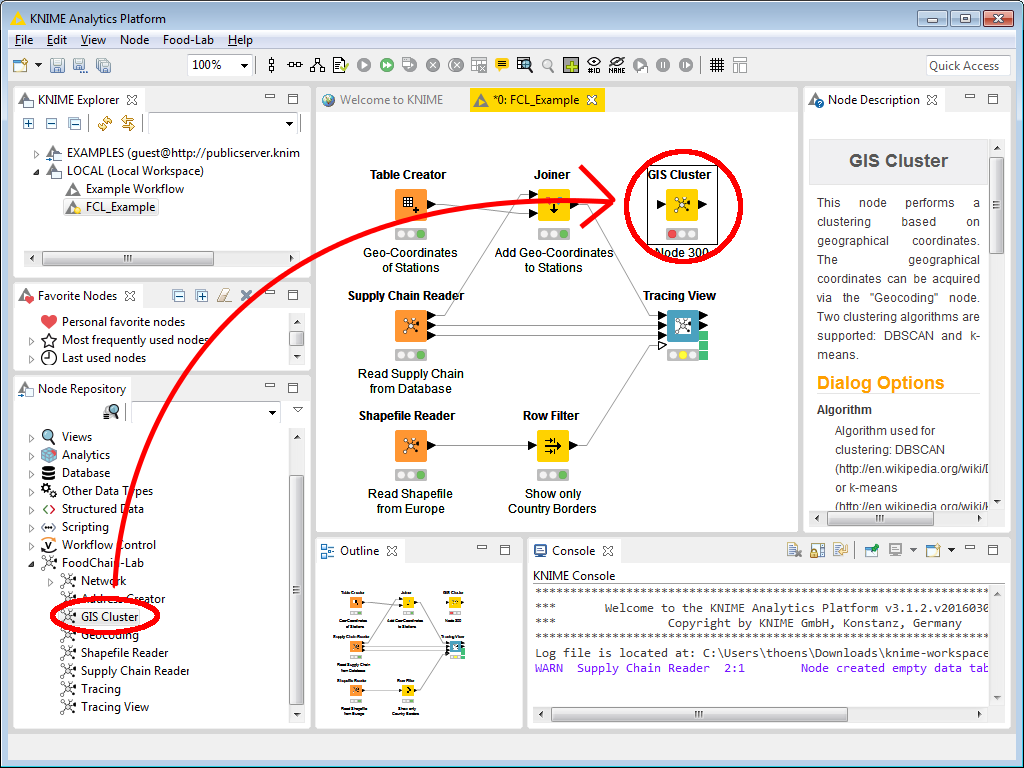
\includegraphics[height=0.6\textheight]{2.png}
	\end{center}
	\begin{itemize}
		\item Drag the \textbf{GIS Cluster} node from \textbf{FoodChain-Lab} in the \textbf{Node Repository} to the \textbf{Workflow Editor}.
	\end{itemize}
\end{frame}

\subsection{3}
\begin{frame}
	\begin{center}
  		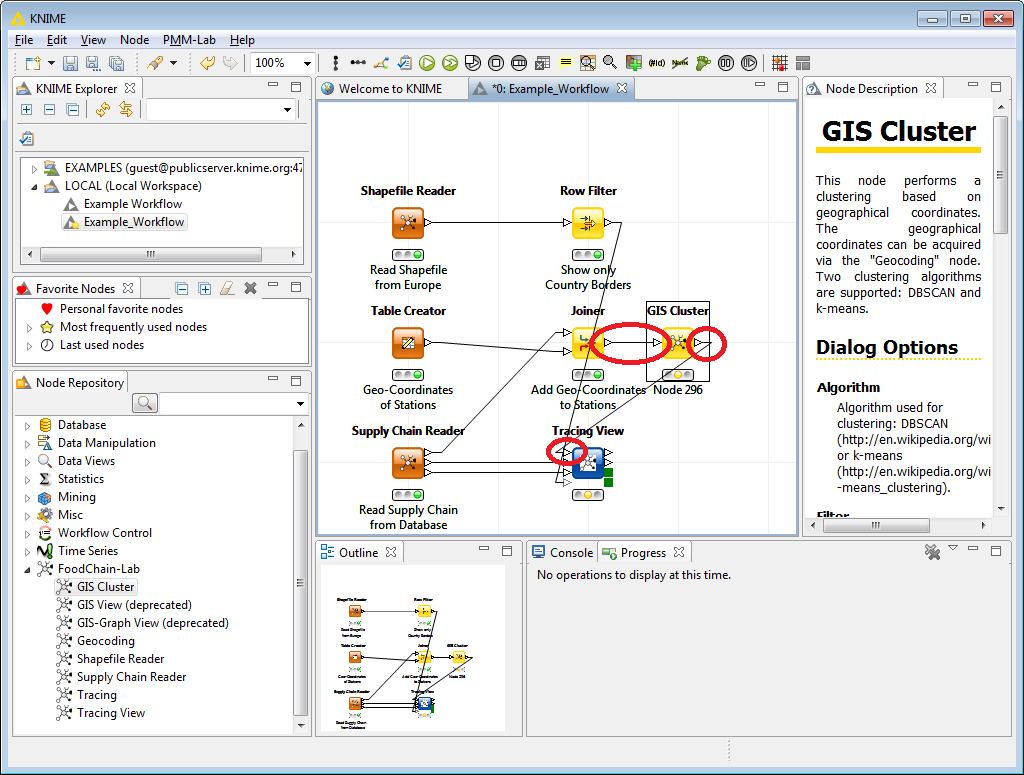
\includegraphics[height=0.6\textheight]{3.png}
	\end{center}
	\begin{itemize}
		\item Connect the output of \textbf{Joiner} to the input of \textbf{GIS Cluster}.
		\item Connect the output of \textbf{GIS Cluster} to the first input of \textbf{Tracing View}.
		\item Double click on the \textbf{GIS Cluster} node to open its dialog.
	\end{itemize}
\end{frame}

\subsection{4}
\begin{frame}
	\begin{center}
  		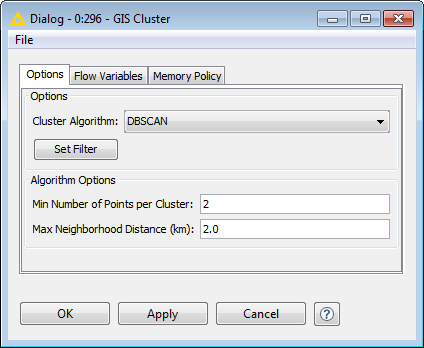
\includegraphics[height=0.6\textheight]{4.png}
	\end{center}
	\begin{itemize}
		\item In this dialog you can set up an algorithm for geographical clustering based latitude and longitude.
		\item Click on \textbf{Set Filter} to define which stations should be clustered.
	\end{itemize}
\end{frame}

\subsection{5}
\begin{frame}
	\begin{center}
  		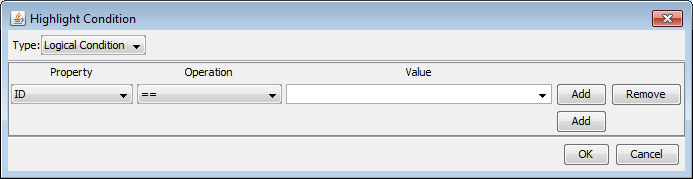
\includegraphics[width=0.9\textwidth]{5.png}
	\end{center}
	\begin{itemize}
		\item You should see this dialog now.
	\end{itemize}
\end{frame}

\subsection{6}
\begin{frame}
	\begin{center}
  		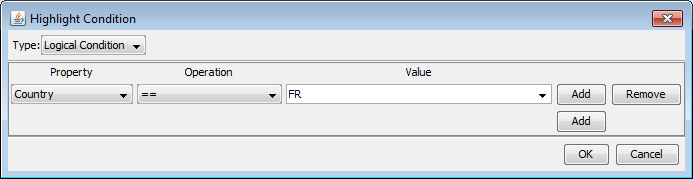
\includegraphics[width=0.9\textwidth]{6.png}
	\end{center}
	\begin{itemize}
		\item For our clustering we only want to use the French stations, since most primary producers in this data set are French.
		\item Select "Country" as \textbf{Property} and "FR" as \textbf{Value} and press \textbf{OK}.
	\end{itemize}
\end{frame}

\subsection{7}
\begin{frame}
	\begin{center}
  		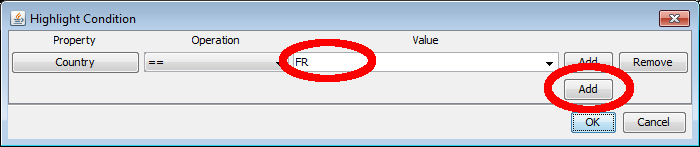
\includegraphics[height=0.6\textheight]{7.png}
	\end{center}
	\begin{itemize}
		\item Set the \textbf{Max Neighborhood Distance} to 100km. That means two stations with distance of less than 100km are put into the same area.
		\item Press \textbf{OK}.
	\end{itemize}
\end{frame}

\subsection{8}
\begin{frame}
	\begin{center}
  		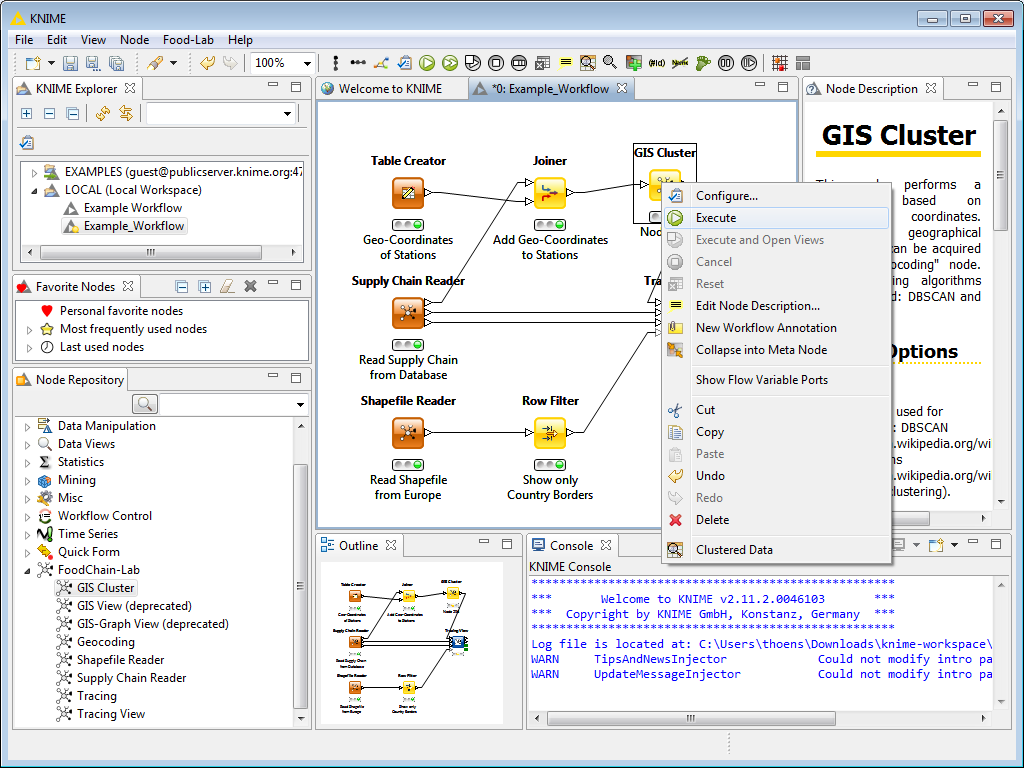
\includegraphics[height=0.6\textheight]{8.png}
	\end{center}
	\begin{itemize}
		\item Right click on \textbf{GIS Cluster} to open its context menu and select \textbf{Execute} to execute the node.
		\item The results of the clustering are put into the \textbf{ClusterID} column. This column will be used in the \textbf{Tracing View}.
	\end{itemize}
\end{frame}

\subsection{9}
\begin{frame}
	\begin{center}
  		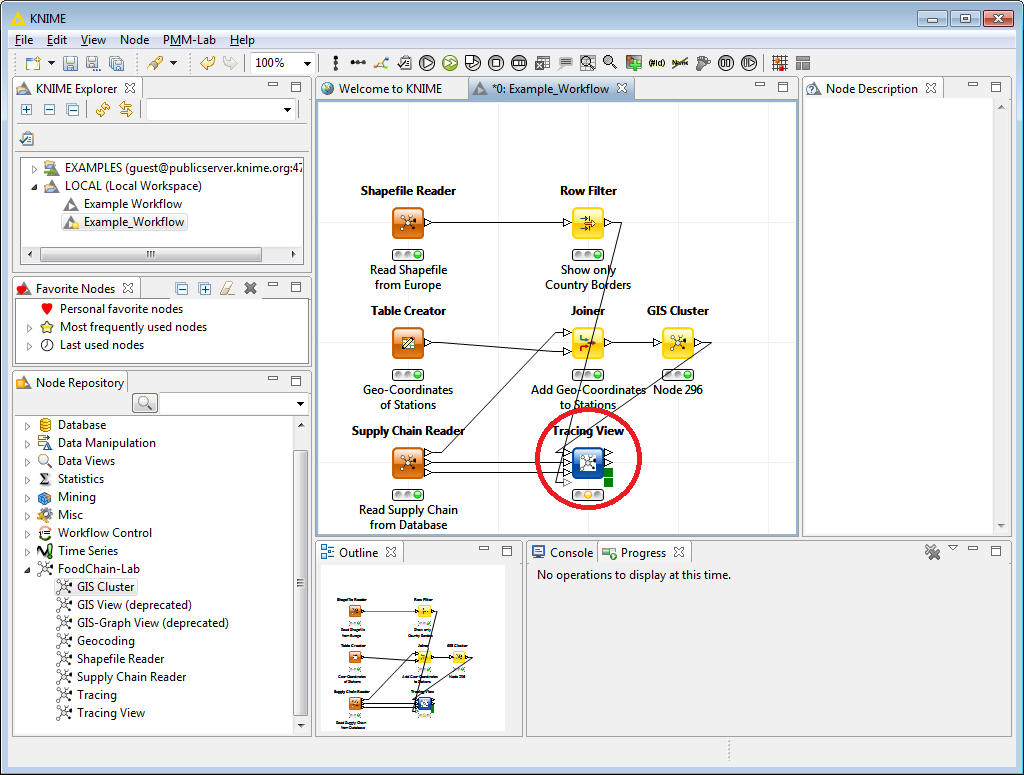
\includegraphics[height=0.6\textheight]{9.png}
	\end{center}
	\begin{itemize}
		\item Open the \textbf{Tracing View} by double-clicking on it.
	\end{itemize}
\end{frame}

\subsection{10}
\begin{frame}
	\begin{center}
  		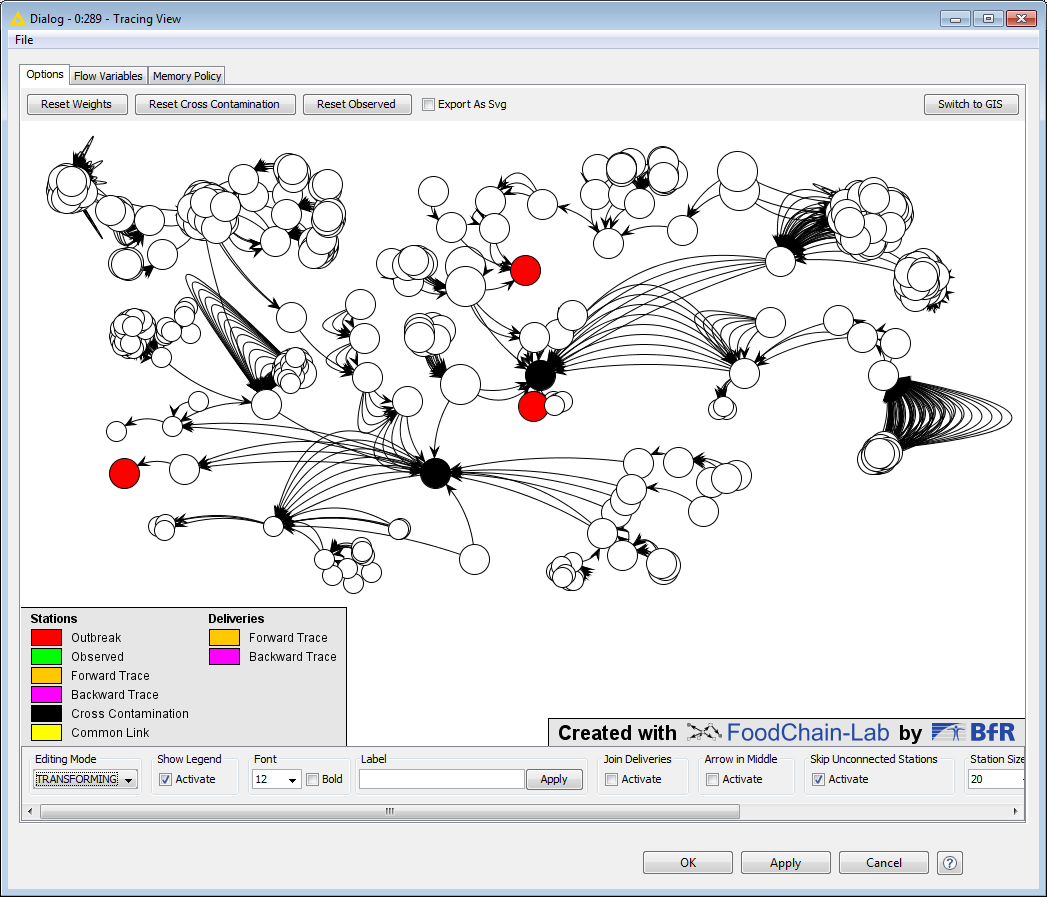
\includegraphics[height=0.6\textheight]{10.png}
	\end{center}
	\begin{itemize}
		\item A window showing the delivery network should open now.
	\end{itemize}
\end{frame}

\subsection{11}
\begin{frame}
	\begin{center}
  		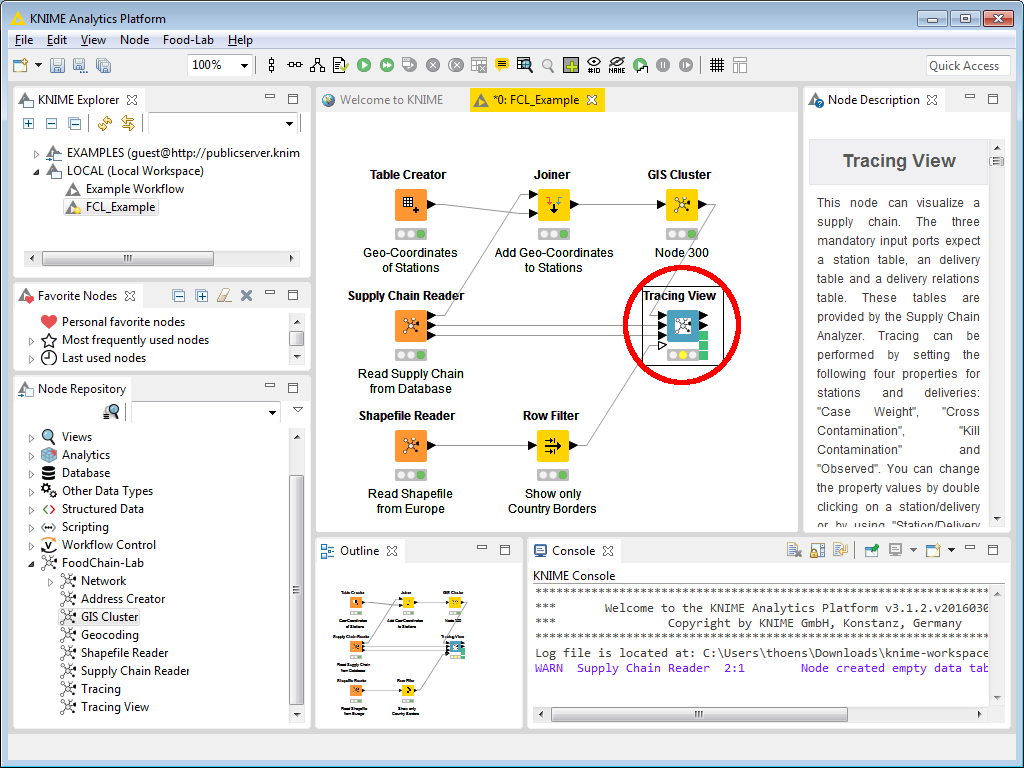
\includegraphics[height=0.6\textheight]{11.png}
	\end{center}
	\begin{itemize}
		\item Right click in the graph to open the context menu and select \textbf{Collapse by Property}.
	\end{itemize}
\end{frame}

\subsection{12}
\begin{frame}
	\begin{center}
  		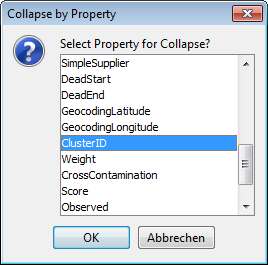
\includegraphics[height=0.5\textheight]{12.png}
	\end{center}
	\begin{itemize}
		\item The clustering will be done based on the results of the \textbf{GIS Cluster} node.
		\item Select \textbf{ClusterID} and press \textbf{OK}.
	\end{itemize}
\end{frame}

\subsection{13}
\begin{frame}
	\begin{center}
  		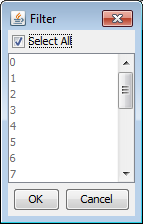
\includegraphics[height=0.5\textheight]{13.png}
	\end{center}
	\begin{itemize}
		\item Just press \textbf{OK}, since we do not want to exclude any area.
	\end{itemize}
\end{frame}

\subsection{14}
\begin{frame}
	\begin{center}
  		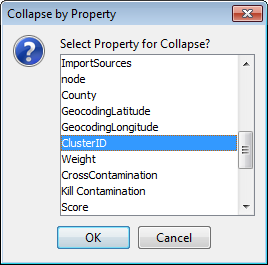
\includegraphics[height=0.6\textheight]{14.png}
	\end{center}
	\begin{itemize}
		\item All French stations have been clustered to areas.
		\item Each selected station (blue circle) is an area in France.		
	\end{itemize}
\end{frame}

\subsection{15}
\begin{frame}
	\begin{center}
  		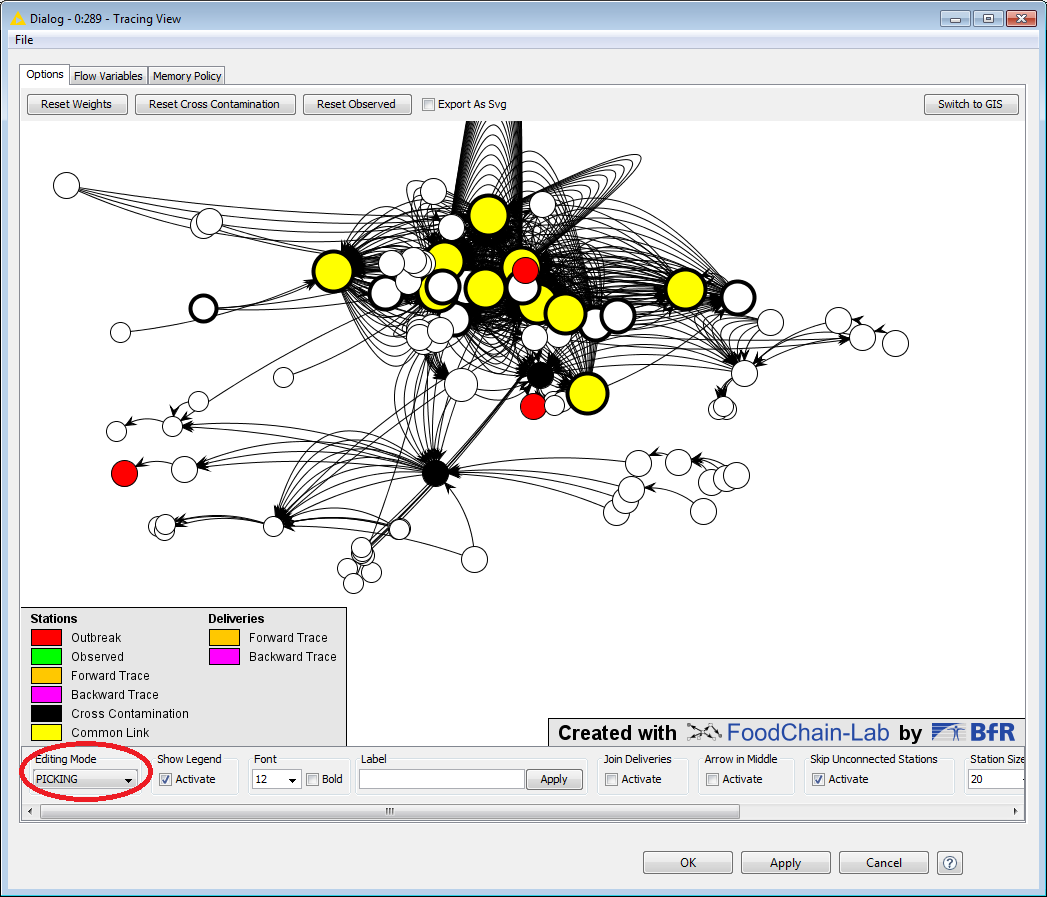
\includegraphics[height=0.6\textheight]{15.png}
	\end{center}
	\begin{itemize}
		\item Select "PICKING" as \textbf{Editing Mode} and click in the graph to unselect all stations.
		\item You can now see, that some of the stations are yellow. That means, that these stations (French areas) are connected to all outbreak spots (red circles).
	\end{itemize}
\end{frame}

\subsection{16}
\begin{frame}
	\begin{center}
  		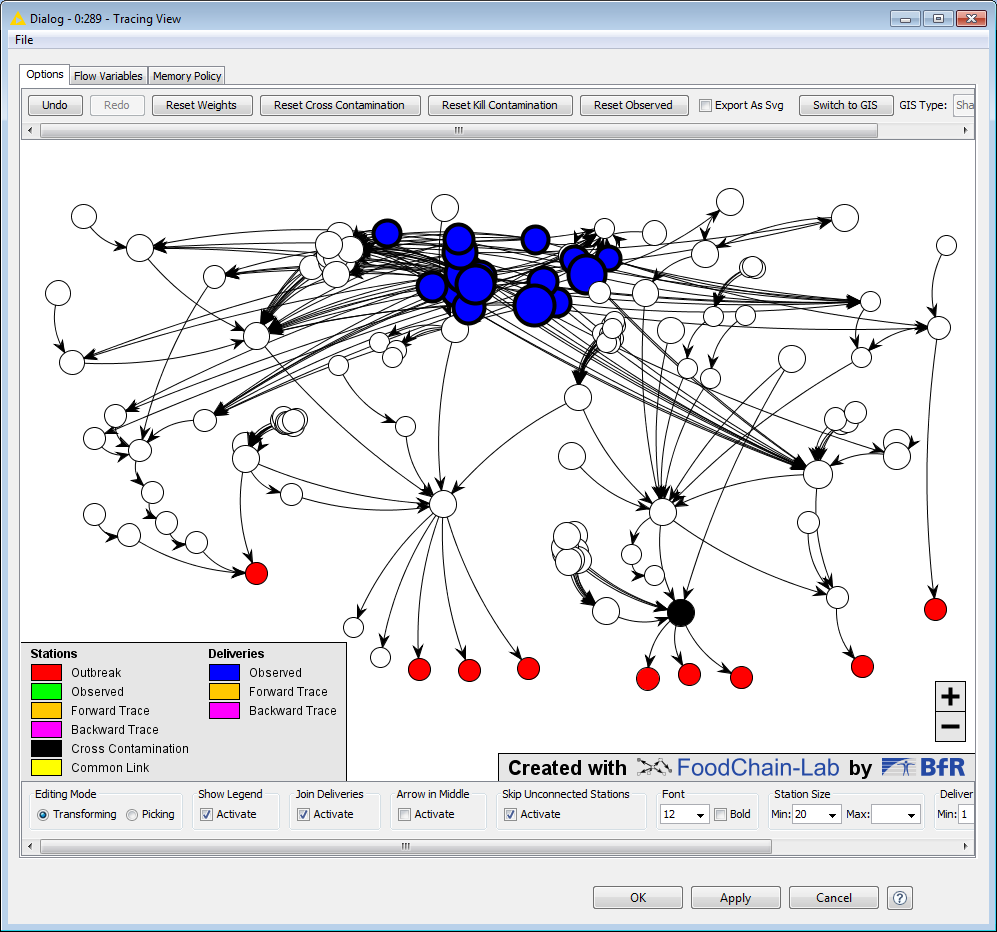
\includegraphics[height=0.6\textheight]{16.png}
	\end{center}
	\begin{itemize}
		\item Since the graph looks confusing now, we should reapply the layout algorithm.
		\item Right click in the graph and select \textbf{Apply Layout $>$ Fruchterman–Reingold} in the context menu.
	\end{itemize}
\end{frame}

\subsection{17}
\begin{frame}
	\begin{center}
  		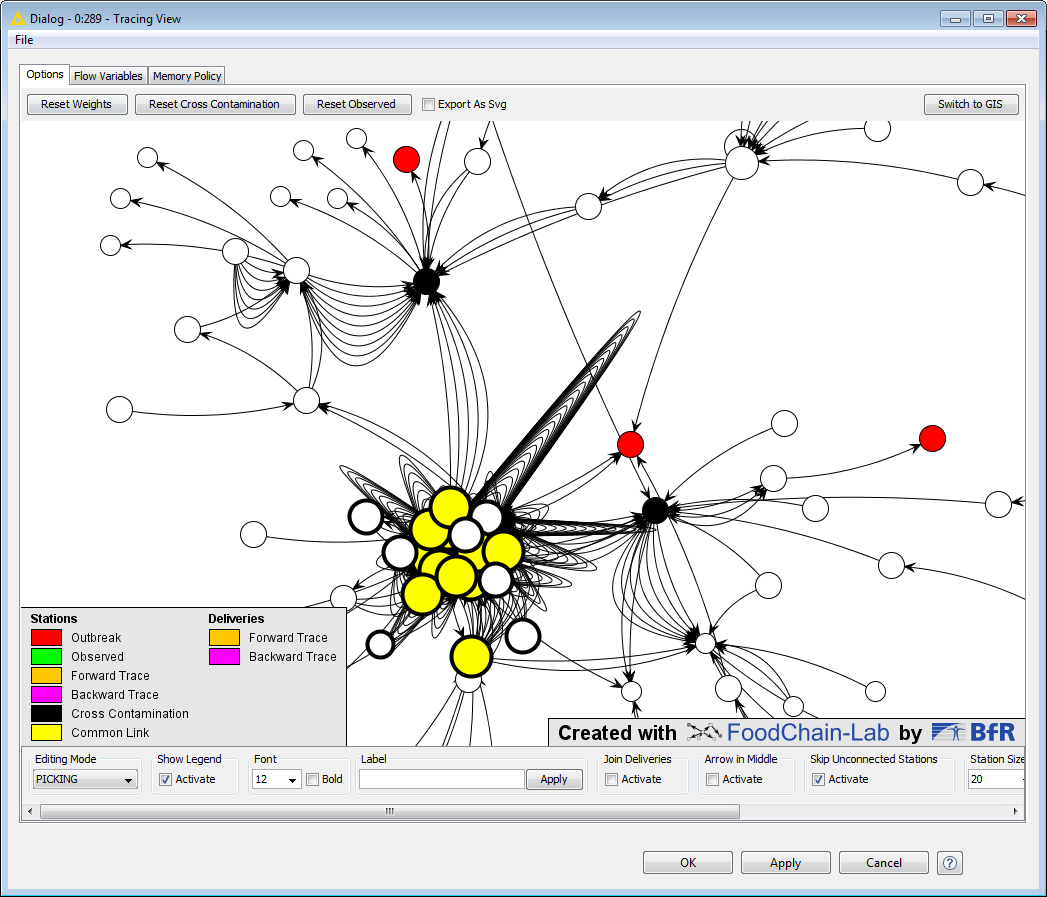
\includegraphics[height=0.6\textheight]{17.png}
	\end{center}
	\begin{itemize}
		\item The stations should be arranged in better way now.
		\item The algorithm is not deterministic, therefore your result will look different from the screenshot.		
	\end{itemize}
\end{frame}

\subsection{18}
\begin{frame}
	\begin{center}
  		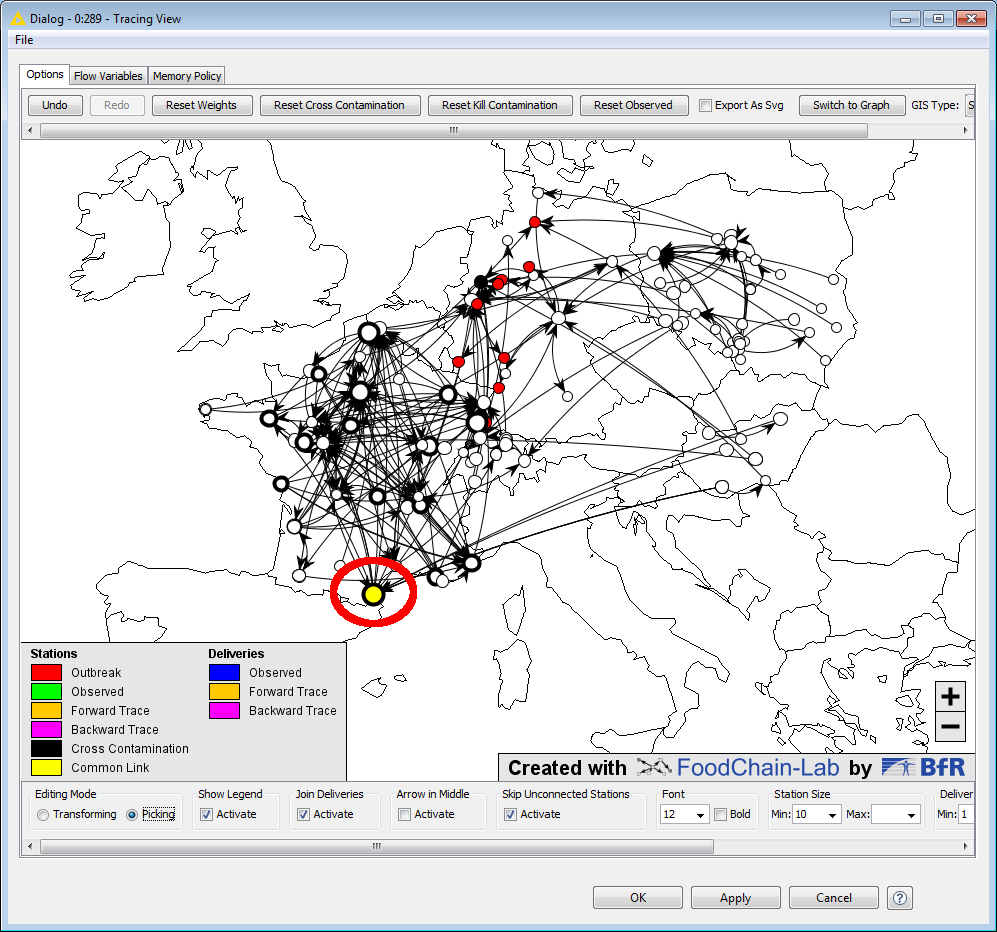
\includegraphics[height=0.6\textheight]{18.png}
	\end{center}
	\begin{itemize}
		\item After applying the layout algorithm some stations might be outside the visible area.
		\item To see the whole graph select "TRANSFORMING" as \textbf{Editing Mode} and zoom/move the graph by using the mouse wheel and the left mouse button (works as in Google Maps).
	\end{itemize}
\end{frame}

\end{document}